\chapter{Background}

This chapter will be used to introduce some basic terminology as well as some basic arguments on why carbon-aware scheduling is useful.

\paragraph{The composition of the public grid}
The public grid is made up of many energy producers. This \emph{energy mix} is composed of different sources: low-carbon technologies like solar, wind, or hydroelectricity and carbon-intensive sources like coal, gas, or oil. 

Figure \ref{fig:energy_mix} shows one such energy example, for a specific location, in this case Germany.
As it is summer, solar production makes up large amount of power at that time. Germany is further interesting in the sense, that it is a country that has no nuclear power stations anymore.

\begin{figure}
    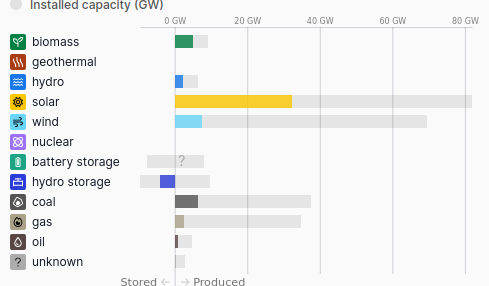
\includegraphics[width=\linewidth, height=200pt]{images/2_background2024-08-20-15-28-19.png}
    \caption[short]{An example snapshot of the energy mix in Germany, at DATE}
    \label{fig:energy_mix}
\end{figure}

Over the day, the demand and supply for power changes. Carbon-efficient sources will generally follow the weather: Solar production follows the amount of sun shining and thus follows a \emph{diurnal} rhythm over the day. Wind and hydroelectricity will also depend on the weather. 
Nuclear energy is generally also considered carbon-efficient, but is generally not useful for carbon-efficient scheduling as the amount of energy produced from is generally stable throughout \todo{QUOTATION NEEDED, maybe use look in on of the related work papers} the day, meaning that there is little use in deferring work to a later time. 

As near-time weather predictions have high accuracy, this enables X.\todo{QUOTATION NEEDED}

Thus, at each point in time the amount of CO2 per unit of electric power can be determined by averaging the amount of power each source supplies to the grid and how much carbon it emits. Figure \ref{fig:carbon_curve} is an example X-day timeframe of the carbon-curve.

\begin{figure}
    \missingfigure{The carbon curve for a few countries at the same time Germany, France, and Poland, }
    \caption[short]{Carbon in per unit of energy in select countries}
    \label{fig:carbon_curve}
\end{figure}

\paragraph{Power grid Signals}
Carbon-aware scheduling commonly works two possible metrics or signals: the \emph{average emissions} are the metric describing the amount of carbon per unit of energy, basically what has been used in the text so far. Another metric is the \emph{marginal emissions}, answering the question of "if more energy is used at this point in time, how much carbon would that cost?". 
The answer to that question is usually that non-renewable power plants have to increase production as renewable sources cannot increase production to meet demand (as the sun and wind intensity are set by the weather). 
Going by the marginal metric, any kind of carbon aware scheduling would be pointless, as any work at any point in time would result in the same increase of carbon. 
Thankfully, there are secondary reasons that would render carbon-aware scheduling useful. One of them are is \emph{curtailment}. 
This encompasses any methods that reduce the amount of produced renewable energy. As the power grid always needs to have a balance between demand and production, curtailment methods such as turning of wind turbines, selling power at a loss, or charging batteries may be used. 
Carbon aware scheduling via the average emissions signal, would lower the amount of curtailment needed, as demand for energy would increase at those times.
Another argument can also be made\todo{Find the quote} that by increasing power demand during times when renewable production is high, energy producers would be "signalled" that there is demand for renewable energy.
Lastly, as renewable energy is generally cheaper in production than non-renewable energy\todo{Need a citation here!}, scheduling work on low carbon-periods coincides with cheaper energy prices as well. While this would not reduce costs on most energy contracts, there are also some contracts that use dynamic pricing \footnote{One example for dynamic pricing would be \emph{Tibber}: \url{https://tibber.com/de}}

\paragraph{Types of work in a datacenter} According to \cite{tanenbaum_operating_2006}, there are 3 environments in which scheduling may take place. \emph{Batch systems} describe environments in which there is no user interaction.
A user may submit their job, and it would be executed according to the scheduler at some point in time. \todo{Does this need more examples?}
On the contrary, in \emph{interactive} settings, a user would be interacting with the system "live", and would thus expect quick responses to their inputs. 
The last environment would be a \emph{real time} system. There deadlines and predictability would dictate how a scheduler would operate.

For this work's topic, carbon-aware scheduling, only batch systems will be looked at as they allow more freedom to the times of scheduled jobs. 

\todo{I could also add more stuff about metrics and so on, but I am not using them yet in my implementation}

Which metrics are there POI-A, etc.

\paragraph{Power intake of a computer}
As there will be power measurements in \ref{sec:power_measurements}, some basic understanding of energy and power used for computation will be provided:
\begin{itemize}
    \item I could mostly borrow from the EBRH slides; there is some base power needed that is correlated to the hardware (dynamic and static energy)
    \item this also depends on frequency (which is why later we set our CPU frequency to some hard coded value [or do not do that in the case of my GPU lol])
    \item basically, use this paragraph to outline all things we take care of in my power measurements
\end{itemize}